\documentclass[11pt,fleqn]{article} 
\usepackage[margin=0.8in, head=0.8in]{geometry} 
\usepackage{amsmath, amssymb, amsthm}
\usepackage{fancyhdr} 
\usepackage{palatino, url, multicol}
\usepackage{graphicx} 
\usepackage[all]{xy}
\usepackage{polynom} 
\usepackage{pdfsync}
\usepackage{enumerate}
\usepackage{framed}
\usepackage{setspace}
\usepackage{array,tikz}
\pagestyle{fancy} 
\lfoot{UAF Calculus 1}
\rfoot{review functions }

\begin{document}
\renewcommand{\headrulewidth}{0pt}
\newcommand{\blank}[1]{\rule{#1}{0.75pt}}
\renewcommand{\d}{\displaystyle}
\vspace*{-0.7in}
\begin{center}
  \large \sc{Worksheet: Review of Functions }
\end{center}
Goals:
\begin{itemize}
\item How to think about and use function notation and terminology.
\item A list of functions to know.
\item Some practice putting these together.
\end{itemize}
\begin{enumerate}
\item The notation $y=f(x)$ means\\
\vspace{1in}
\item  Let $f(x) = 10-3x^2.$ Expand the expressions below and collect like terms. 
\begin{multicols}{2}
 \begin{enumerate}
      \item $\d f(5)$\\
      
	\vspace{1in}
	
      \item $\d f(3a)$\\
      
	\vspace{1in}

      \item $\d 2\left[f(a)\right]^2$\\
      
	\vspace{1in}   
	\columnbreak   
	
	\item $\d f(x+h) $\\
      
	\vspace{1in}      
	
	\item $\d f(x) + h$\\
      
	\vspace{1in}     
	 \end{enumerate}
\end{multicols}
\newpage
\item Below is a list of expressions you should be able to graph instantly. Your graphs should always include any $x$- and $y$-intercepts, asymptotes, and clearly indicate end behavior.
\begin{center}
$y=x$, \quad y=b, \quad $x=a$, \quad$y=x^2,$ \quad$y=x^3,$ \quad$y=\frac{1}{x}$,\quad $y=\frac{1}{x^2}$, \quad $y=\sqrt{x}$, \quad $y=\sqrt[3]{x}$\\ $y=|x|,$\quad $y=e^x$, \quad $y=2^x$,  \quad$y=e^{-x}$, \quad$y=\ln x$,\quad$y=\log_{10}(x)$
\end{center}
\vfill
Include domain and range!
\newpage
\begin{center} Some Extra Practice \end{center}
\item Write the equation of the line through the point $(2,-5)$ that is parallel to the line $4x+3y=17.$
\vfill
\item Find the domain and range of $f(x) = 4+\sqrt{11 - x}.$ Give your answers in interval notation. Explain how you got your answer.
\vfill
\newpage
\item Sketch the graph of $f(x)=\begin{cases} e^x & x \leq 0 \cr 3-x^2 & 0 < x \cr \end{cases}$
\vfill
\item Determine any $x$- or $y$-intercepts for the graphs below.
	\begin{enumerate}
	\item $g(x)=2x^2+13x-7$
	\vfill
	\item $h(x)=\frac{a}{x-b}$ (Assume $a$ and $b$ are fixed positive constants.)
	\vfill
	\end{enumerate}
\item Bonus: Sketch the functions $g$ and $h$ from the previous problem.
\end{enumerate}
\end{document}
%%%%%%%%%%%%
%%%%%%%%%%%%
%%%%%%%%%%%%
Functions can be
represented in a variety of ways. Specifically, there are four that we
will focus on during this course. They are:

\vskip1in


\textbf{Example 1:} (Graphically) Interpreting the graph of a function. The graph of
a function $f$ is shown below. Find the following:

\begin{quote}
  \begin{multicols}{2}{
      % make sure you added \usepackage{enumerate}
      \vspace*{-0.55in}
      \begin{enumerate}[a)]
      \item $f(1)$ and $f(5)$
      \item the domain of $f$
      \item the range of $f$
      \item For which value of $x$ is $f(x) = 4$?
      \item Where if $f$ increasing?
\columnbreak
\begin{center}
  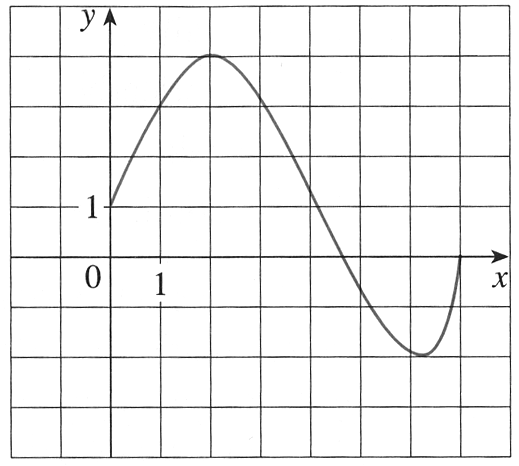
\includegraphics[width=2.8in]{1-1-fig-6}
\end{center}
      \end{enumerate}}
\end{multicols}
\end{quote}
\vskip0.45in
\item Find the domain if each of the following:


\textbf{Example 2:} (Algebraically) If $f(x) = 3x^2 - x + 2$ find the
following. Are (b) and (c) different? 

\begin{quote}
  \begin{multicols}{2}{
      % make sure you added \usepackage{enumerate}
      \vspace*{-0.45in}
      \begin{enumerate}[(a)]
      \item $f(2)$
\vskip1in
      \item $f(a^2)$
\vskip1in
      \item $[f(a)]^2$
\columnbreak
      \item $\d \frac{f(a+h) - f(a)}{h}$
      \end{enumerate}}
  \end{multicols}
\end{quote}

\vskip2.5in


\textbf{Example 3:} Graph the following functions. Give the domain and
range. 
\begin{quote}
  \begin{multicols}{2}{
      % make sure you added \usepackage{enumerate}
      \vspace*{-0.45in}
      \begin{enumerate}[a)]
      \item $f(x) =
        \begin{cases}
          -1\; &\text{if} \; x \ge 2 \\
          7 - 2x \; & \text{if} \; x < 2
        \end{cases}$

        \begin{flushleft}
          \includegraphics[width=1.9in]{grid-print}
        \end{flushleft}

      \item $f(x) =
        \begin{cases}
          x+1 \; &\text{if} \; x \le - 1 \\
          x^2 \; &\text{if} \; x > -1
        \end{cases}$

           \begin{flushleft}
          \includegraphics[width=1.9in]{grid-print}
        \end{flushleft}
      \end{enumerate}}
  \end{multicols}
\end{quote}
\vskip0.5in
\textbf{Domain of a Function:} 

The \textbf{domain} of a function is the set of all possible values of
the input. One can find the domain of a function from a picture, but
it is also possible to do so from an equation. In many instances it is
easier to think about what operations are illegal and leave out the
numbers that break these operations. Remember, 

\begin{enumerate}
\item Thou shalt not divide by \blank{1in}. Set the \blank{1.5in}
  equal to zero. Leave these numbers out. 
\item Thou shalt not square root \blank{1in}. Set the stuff under the
  radical \blank{0.25in} zero and solve. Note, solving polynomial
  inqualities is not simple. 
\item Thou shalt not take the logaraithm of \blank{1in}. Set the stuff
  inside the logarithm \blank{0.25in} zero and solve. This process is
  quite similar to \# 2. 
\end{enumerate}


\textbf{Example 3:} Find the domain of each function. Give the domain
using interval notation. 
\begin{quote}
  \begin{multicols}{2}{
      % make sure you added \usepackage{enumerate}
      \vspace*{-0.45in}
      \begin{enumerate}[(a)]
      \item $f(x) = \d \frac{1}{x^4 - 16}$
      \item  $f(x) = \sqrt{x} + \sqrt{11 - x}$
      \end{enumerate}}
  \end{multicols}
\end{quote}
\vskip2in

\newpage
\textbf{Example 4:} Find the domain of each function. Give the domain
using interval notation. 
\begin{quote}
  \begin{multicols}{2}{
      % make sure you added \usepackage{enumerate}
      \vspace*{-0.45in}
      \begin{enumerate}[a)]
      \item $g(x) = \ln( x^2 - 4 )$
      \item $h(x) = \frac{1}{\sqrt{x^2 - 5x - 6}}$
      \end{enumerate}}
  \end{multicols}
\end{quote}


\vskip1.5in

\textbf{Example 6:} A rectangular storage container with an open top
has a volume of 10 $m^3$. The length of its base is twice the
width. Materials for the base cost \$10 per square meter and material
for the sides cost \$6 per square meter. Express the cost of materials
as a function of the width of the base.  Give the domain of the
function. 
\vskip2.5in

\subsection*{Symmetry}

\begin{itemize}
\item A function $f(x)$ is called even if \blank{1in}. An example is
  $f(x) = $ \blank{0.5in}. Even functions are symmetric about
  \blank{1in}.
\item A function $f(x)$ is called odd if \blank{1in}. An example is
  $f(x) = $ \blank{0.5in}. Odd functions are symmetric about the
  origin. 
\end{itemize}

\textbf{Example 7:} Determine whether the following functions are
even, odd, or neither. 


  \begin{multicols}{3}{
      % make sure you added \usepackage{enumerate}
      \vspace*{-0.45in}
      \begin{enumerate}[a)]
      \item $g(x) = e^x + 1$
      \item $f(x) = 1 + 3x^2 - x^4$
      \item $f(x) = \frac{x}{x^2+1}$
      \end{enumerate}}
  \end{multicols}




\end{document}